\documentclass[a4paper, titlepage]{article}

\usepackage{microtype}
\usepackage{amsmath}
\usepackage{index}
\usepackage{fancyhdr}
\usepackage[hidelinks]{hyperref}
\usepackage{float}
\usepackage{tabularx}
\usepackage{tikz}
\usepackage{graphicx}
\usepackage{ltablex}
\usepackage[left=4cm,right=4cm]{geometry}
\usepackage{subcaption}
\usepackage{listings}


\hypersetup{
	colorlinks=true,
	linktoc=all,    
	linkcolor=black,
	%linktocpage
}

\usetikzlibrary{positioning, shapes, calc}

\renewcommand{\lstlistingname}{Algorithm}% Listing -> Algorithm

\begin{document}

\title{}
\author{Alex Greig}
\begin{titlepage}
	\centering
	
\includegraphics[width=0.5\textwidth]{sta-logo.png}\par
	\vspace{1.5cm}
	\noindent\rule{12cm}{0.07cm} \\
	\vspace{0.2cm}
	{\huge{\textbf{Nodepaths\\Project Portfolio - Task 1}}\\}
	\vspace{0.2cm}
	\noindent\rule{12cm}{0.07cm} \\
	\vspace{1.5cm}
	{\LARGE{\emph{By Alex Greig}}} \\
	\vspace{1.5cm}
	{\large{\emph{ \today}}}
	\vfill
\end{titlepage}

\tableofcontents
\vfill
\section{Project Portfolio}

\subsection{Problem Definition}
The problem with today's internet is the control large corporations have over information transmission, enabling data to be lost, monetized, or given to the government, all without users knowing. Another problem of the internet is the inherent security flaws associated with centralised control; that is, its ability to be hacked. The final problem is the inequality of the internet as large populations throughout the world are unable to access the internet, with access they would be able to receive better educational resources, progressing humanity forward. \\


The application that I am creating is called Nodepaths, and it is important for the consumer market as it will provide high security to user's data and a network that is robust and resistant to problems allowing for secure data transfer between devices globally, solving the problems above. The application will have a significant effect on the way we use the internet and allow users to share, communicate and complete complex computational tasks efficiently and securely. The application will be a decentralised network that uses peer-to-peer architecture and mesh topology, allowing any machine capable of connecting to a network to join and become a "node". The application will also include the feature of Wi-Fi peer to peer transmission allowing for nodes to be connected by Wi-Fi radio waves eliminating costs of telecommunication services, however, if users cannot be connected by the mesh then cellular internet is available. This information will be encrypted, end to end. The mesh network will relay data and messages using a wireless ad-hoc network, where data is propagated along a path by hopping from node to node until it reaches its destination. The paths will be calculated based on the Ad-Hoc On Demand Vector Routing protocol (AODV), a routing protocol that determines and maintains routes whenever they are required. \\

The application that I am creating, Nodepaths, will have three main functions. The first is creating a user, to do this it will need to create identification. The application will create a public and private key using the Curve25519 elliptic curve in conjunction with the Diffie–Hellman key agreement scheme and the Advanced Encryption Standard, then a psuedo-random IPv4 Address and finally validate a username that has been entered by the user. The second function of Nodepaths is to transfer data, normally messages, over a wireless ad-hoc network to another node. The final main function of the application will be to give users the ability to add new nodes (friends) to the application allowing them to select friends that they want to text to. These three functions when integrated will provide the foundation for a user-friendly text messaging application that runs on a decentralised, distributed network. Although the functions may seem simple or basic the underlying backend behind a network of this caliber is complex; to function, innovative solutions are needed. \\

Future improvements and upgrades to the application will include the implementation of Blockchain technology to provide digital transactions and a cryptographic wallet on the application, eliminating the need for banks and other financial institutions. In the future, the application may also provide assistance to disadvantaged communities as it would give them communication without the cost of telecommunication services.

\subsection{Input, Output and Processes Diagram}
	\vspace{2mm}
	\begin{tabularx}{\linewidth}{ |*{3}{X|}}
	\hline 
	\multicolumn{1}{|>{\centering}X|}{Input} &
	\multicolumn{1}{>{\centering}X|}{Processing} &
	\multicolumn{1}{>{\centering}X|}{Output} \\
	\hline\hline
	The user opens the application for the first time, and they are asked to input a username. & The application calculates a pseudo-random number with a uniform distribution to create a IPv4 address in the range of 192.168.1.0 to 192.168.254.255. It then creates an asymmetric key pair, a private and public key that will be used for identification of nodes and end-to-end encryption of data transmissions. It then takes the username that was inputed and validates it, checking that the length is between 5 and 20 characters and doesn't contain any special characters. The username, the IPv4 address and the key pair are stored securely in the phone storage & If a username was inputted that doesn't meet the required validation then the user will be redirected to enter another username. A loading screen is displayed with text saying, ``Setting up Profile and Configuration." This happens while waiting for operations to be complete, then welcome text appears when done and a main menu appears. \\
	\hline\hline
	The user selects the option on the main menu, ``Search for users on the network." & Using the mobile phone's API for peer-to-peer Wi-Fi connections it sends out a Wi-Fi signal and also listens for incoming Wi-Fi connections. It sends a data packet on the network containing the username and searches for users with the same name. If there are multiple users with the same username then the user can select the profile they want. The two nodes establish a connection and communication is available & The user is prompted with the different users that have the username they searched, it then displays the ability to add them. If they add a node as a friend, the text, ``Successfully added [username] as a friend" will be displayed.  \\
	\hline\hline
	The user scans a QR code of another user. & The QR code is a representation of the public key, IP address and username of a user and when it is scanned, it is saved onto the mobile phone's storage & Display text, "Successfully added [username] as a friend"  \\
	\hline\hline
	When in the chat section of the application the user selects a user to message, they then send a text to them. & The application, utilising the ad-hoc on-demand vector routing protocol will flood the network with Route Request Packets via UDP, if the route is found then a Route Reply packet will be sent, this contains the shortest path between users. When the path is created using TCP, the public keys will be exchanged. The message will be encrypted with the other user's public key and transmitted across the network. The message will be validated to make sure the packet size isn't larger than 100 MB. & Once the message has been sent, the message on the user's screen goes blue, displaying to the user that the message has been transmitted. \\
	\hline\hline
	Within the profile section of the application the user can select to add a photo to their profile. & The application will open the default picture viewing application on the phone and allow the user to select a picture. The user can scale the photo to fit inside a circle with diameter of 1000 pixels. & The default photo viewing application will be displayed, then the text, "Successfully added the profile picture," will be displayed once the picture is scaled and fitted to the profile picture template.\\
\hline
\end{tabularx}

\subsection{Context and Data-flow Diagrams}
\vspace{2cm}
\begin{figure}[H]
\caption{Context Diagram}
\vspace{1cm}
\centering
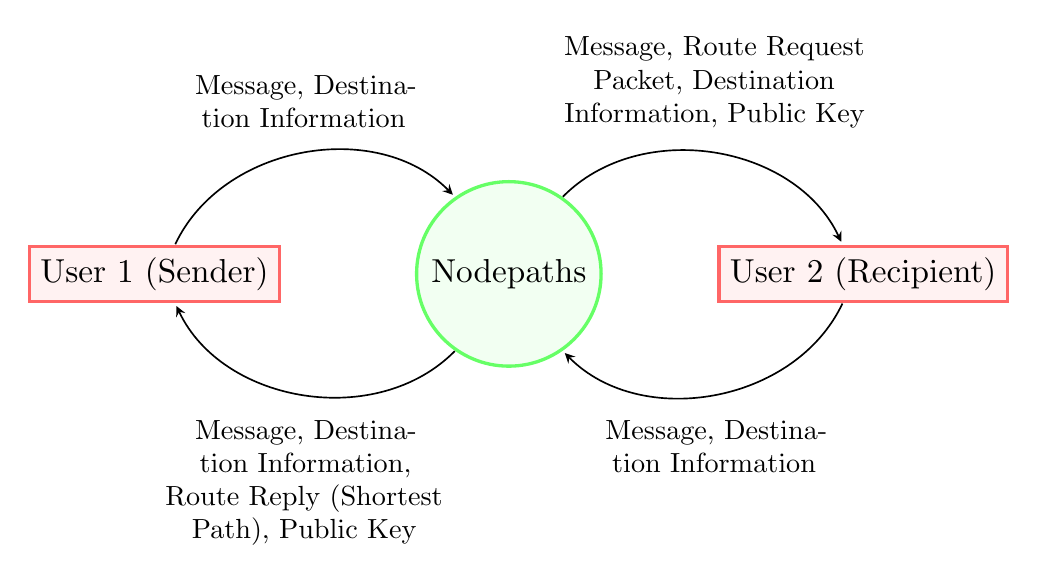
\begin{tikzpicture}[
roundnode/.style={circle, scale = 1.2, draw=green!60, fill=green!5, very thick, minimum size=7mm},
squarednode/.style={rectangle, scale = 1.2, draw=red!60, fill=red!5, very thick, minimum size=5mm},
to/.style={->,>=stealth,shorten >=1pt,semithick},
]
%nodes
\node[squarednode](e1) at (-4.5, 0) {User 1 (Sender) };
\node[roundnode](p) at (0,0) {Nodepaths};
\node[squarednode](e2) at (4.5, 0) {User 2 (Recipient)};
%connections
\draw[to] (e1) to [bend left = 55] node[align=center, text width = 4cm, above = 0.2cm] {Message, Destination Information}(p);
\draw[to] (p) to [bend left = 55] node[align=center,text width = 4cm, midway, below = 0.2cm] {Message, Destination Information, Route Reply (Shortest Path), Public Key}(e1);
\draw[to] (p) to [bend left = 55] node[align=center,text width = 4cm, midway, above = 0.2cm] {Message, Route Request Packet, Destination Information, Public Key}(e2);
\draw[to] (e2) to [bend left = 55] node[align=center,text width = 4cm, midway, below = 0.2cm] {Message, Destination Information}(p);
\end{tikzpicture}
\end{figure}

\begin{figure}[H]
\caption{Data Flow Diagram}
\vspace{1cm}
\centering
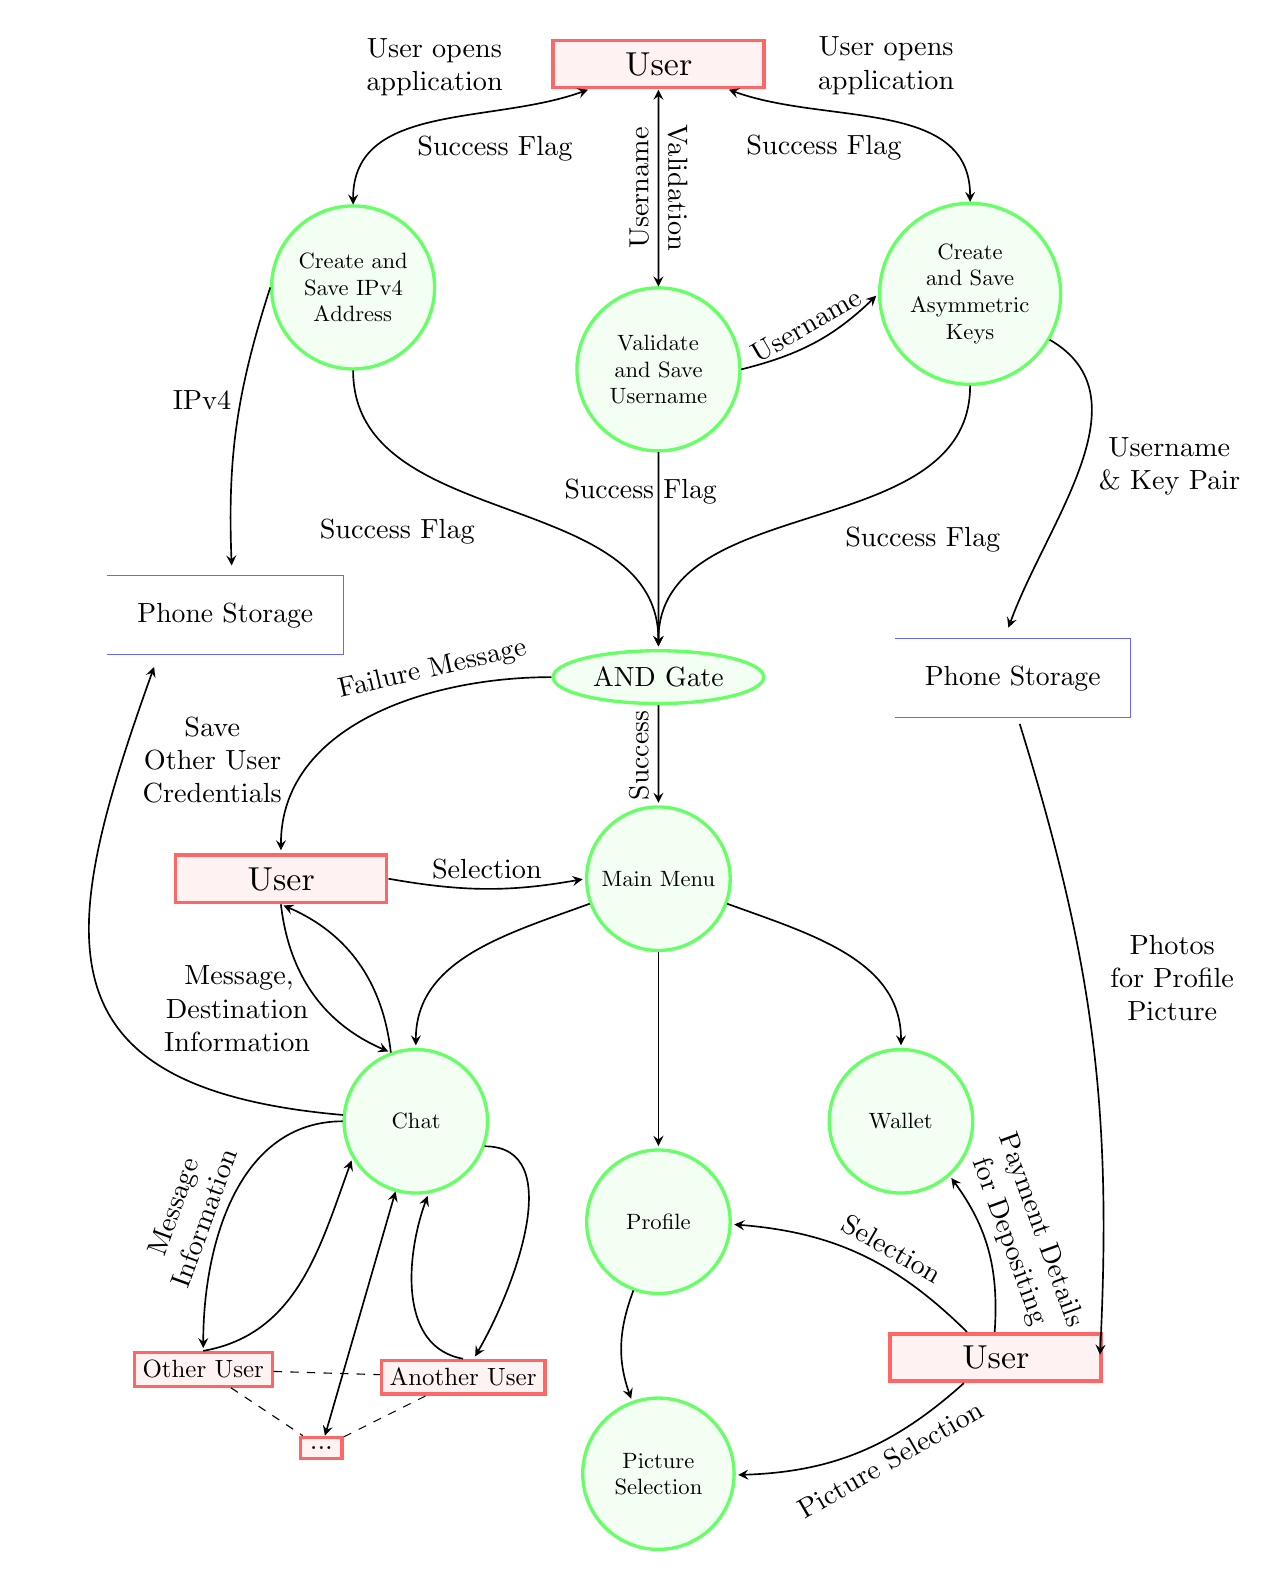
\begin{tikzpicture}[node distance = 2.5cm,
process/.style={circle, scale = 0.8, align=center, text width = 2cm, draw=green!60, fill=green!5, very thick, minimum size=7mm},
entity/.style={rectangle, scale = 1.2, align=center, text width = 2cm, draw=red!60, fill=red!5, very thick, minimum size=5mm},
path/.style={->,>=stealth,shorten >=1pt,semithick},
]

\tikzset{
  pics/datastore/.style args={#1,#2, #3}{
     code={
	     \draw [draw=blue!60] (0,0) -- (3,0) -- (3,1) -- (0, 1);
	     \node[#3] (#1) at (1.5,0.5) {#2};
     }
  }
}

%Nodes
\node [entity] (user) {User};
\node [process] (c_ip) [below left = of user]{Create and Save IPv4 Address};
\node [process] (c_ak) [below right = of user]{Create and Save Asymmetric Keys};
\node [process] (s_username) [below = of user]{Validate and Save Username};
\node [draw, ellipse, draw=green!60, fill=green!5, very thick] (and) [below = of s_username] {AND Gate};
\draw (3, -8.3) pic{datastore={pstore, Phone Storage, black}};
\draw (-7, -7.5) pic{datastore={pstore2, Phone Storage, black}};
\node [process, yshift=-3.2cm] (m_menu) at (and) {Main Menu};
\node [entity] (user2) [left = of m_menu] {User};
\node [process] (chat) [below left = of m_menu] {Chat};
\node [process] (wallet) [below right = of m_menu]{Wallet};
\node [process] (profile)  [below = of m_menu] {Profile};
\node [scale =0.9, yshift = -3.5cm, xshift = -3cm, align=center, draw=red!60, fill=red!5, very thick] (u1) at (chat) {Other User};
\node [scale = 1, yshift = -1cm, xshift = 1.5cm, align=center, draw=red!60, fill=red!5, very thick] (u2) at (u1) {...};
\node [scale =0.9, yshift = 1 cm, xshift = 2cm, align=center, draw=red!60, fill=red!5, very thick] (u3) at (u2) {Another User};
\node [entity, yshift=-2.5cm, xshift = 1cm] (user3) at (wallet) {User};
\node [process, yshift = -4cm] (p-select) at (profile) {Picture Selection};

% Paths

\draw [stealth-stealth, semithick](user) edge[out=200, in=90] node[align=center, midway, text width=2.5cm, above = 0.2cm] {User opens application} node[align=center, pos=0.3, text width=2.5cm, below = 0.2cm] {Success Flag} (c_ip); 
\draw [stealth-stealth, semithick] (user) to node[align=center, text width=2.5cm, midway, rotate = 90, above] {Username} node[align=center, text width=2.5cm, midway, rotate = 270, above] {Validation} (s_username); 
\draw [stealth-stealth, semithick](user) edge[out=340, in=90] node[align=center, midway, text width=2.5cm, above = 0.2cm] {User opens application} node[align=center, pos=0.3, text width=2.5cm, below= 0.2cm] {Success Flag} (c_ak); 

\draw (c_ip) edge[out=270, in=90, path] node[align=center, midway, text width=2.5cm, below left] {Success Flag}(and);
\draw (c_ak) edge[out=270, in=90, path] node[align=center, midway, text width=2.5cm, below right] {Success Flag}(and);
\draw [path] (s_username) to node[align=center, pos=0.2, xshift=-2.25mm] {Success Flag} (and); 
\draw [path] (and) to node[align=center, midway, rotate=90, above] {Success} (m_menu); 
\draw (and) edge[out=180, in=90, path] node[align=center, pos=0.3, above, rotate=13] {Failure Message} (user2);
\draw [path] (user2.0) to [bend right = 10] node[align=center, text width = 4cm, midway, above] {Selection} (m_menu.west);

\draw (m_menu) edge[out=200, in=90, path] (chat); 
\draw (m_menu) edge[out=340, in=90, path] (wallet); 
\draw [path] (m_menu) to (profile); 
\draw [path] (user2.south) to [bend right = 30] node[align=center, pos=0.6, left, text width = 2cm] {Message, Destination Information} (chat.110);
\draw [path] (chat.110) to [bend right = 30] (user2.270);

\draw (chat) edge[out=180, in=90, path] node[align=center, pos=0.6, text width = 2cm, rotate=70, above] {Message Information} (u1);
\draw (u1.north) edge[out=10, in=250, path] (chat.210);
\draw (chat.-20) edge[out=0, in=60, path] (u3);
\draw (u3.north) edge[out=170, in=250, path] (chat.280);
\draw [dashed](u1) -- (u2);
\draw [dashed](u2) -- (u3);
\draw [dashed](u1) -- (u3);
\draw [stealth-stealth, semithick](u2) -- (chat);

\draw [path] (profile) to [bend right = 20] (p-select);
\draw [path] (user3) to [bend right = 20] node[align=center, pos=0.4, above, text width = 3cm, rotate=-30] {Selection} (profile);
\draw [path] (user3) to [bend left = 20] node[align=center, pos=0.4, below, text width = 3cm, rotate=30] {Picture Selection} (p-select);
\draw [path] (user3) to [bend right = 20] node[align=center, pos=0.5, above, text width = 3cm, rotate=-70] {Payment Details for Depositing} (wallet);

\draw [path] (c_ip.west) to [bend right = 10] node[align=center, pos=0.4, xshift=-0.5cm, text width = 3cm] {IPv4} ($(c_ip.west)!3.6cm!(pstore2)$);
\draw [path] (s_username.east) to [bend right = 15] node[align=center, pos=0.5, above, text width = 2cm, rotate=30] {Username} (c_ak.west);
\draw [path] (c_ak) edge[out=330, in=70] node[align=center, pos=0.5, right, text width = 2cm] {Username \& Key Pair} ($(c_ak)!4.3cm!(pstore)$);
\draw [path, transform canvas={yshift=-0.3cm}] (pstore) to [bend left = 10] node[align=center, pos=0.4, right, text width = 2cm] {Photos for Profile Picture} ($(pstore)!8.4cm!(user3.east)$);
\draw [path, shorten >= 0.4cm] (chat) .. controls (-8, -13) and (-7.6, -11) .. node[align=center, pos=0.85, right, text width = 2cm] {Save Other User Credentials} (pstore2.200);
\end{tikzpicture}
\end{figure}

\subsection{Algorithms}

\end{document}

